\documentclass[12pt]{article}
\usepackage[margin=2cm]{geometry}
\usepackage{amsmath}
\usepackage[svgnames]{xcolor}
\usepackage{graphicx}
% \usepackage{hyperref}
\usepackage{longtable}
\usepackage{float}
\usepackage{enumitem}
\begin{document}
	\newcommand{\ssq}{\ensuremath{\sqrt{2}}}
	\newcommand{\um}{\ensuremath{\mu \textrm{m}}}
	\newcommand{\ITF}{\color{Black}2025[I]\ }
	\newcommand{\STT}{\color{Olive}2022[S]\ }
	\newcommand{\TTT}{\color{Olive}2023\ }
	\newcommand{\TWT}{\color{Olive}2022\ }
	\newcommand{\nss}{\vspace*{-1.5em}}
	\newcommand{\linedSection}[1]{%
	\section*{\centering Module #1}
		\hrule
		\vspace*{10pt}
	}
	\newcounter{ct}
	\setcounter{ct}{1}
	\newcommand{\ct}{%
	\arabic{ct}%
	\stepcounter{ct}%
	}
	\title{\vspace*{-1.5cm} VLSI Questions}
	\date{}
	\maketitle
\vspace*{-2cm}
\begin{center}
	Compilation of previous year questions and internal papers \\[12pt]

	([S] -> Supply exam, [I] -> Internal)
\end{center}
\renewcommand{\arraystretch}{1.8}
\linedSection{1}
\begin{longtable}{rp{.86\textwidth}p{1.3cm}}
 & \textbf{Question} & \textbf{asked in} \\
\ct & Describe the process steps of n-well CMOS fabrication with neat sketches &\nss \TWT \\
\ct & Describe the process steps of p-well CMOS fabrication with neat sketches &\nss \ITF \\
\ct & Explain the process steps involved in the nMOS fabrication with neat sketches. &\nss \TWT \ITF \\
\ct & Explain CMOS IC fabrication technology in detail. & \nss \STT \\

\ct & Explain the four approaches involved in the fabrication of CMOS IC technology with neat figures.

{\color{teal} $\rightarrow$ Refers to n-well, p-well, twin tub, SOI}& \nss \TTT \\

\ct & Discuss the Twin tub process in detail. & \nss \STT \\

\ct & Explain Ion implantation process in IC fabrication. & \nss \STT \\

\ct & Describe the various second order MOS device effects in detail. & \nss \TWT \ITF\\

\ct & Discuss any five non-ideal I-V effects that come into play, when the channel length is scaled down to the order of the depletion layer. & \nss \STT \\
\ct & Compare bipolar and MOS/CMOS technologies. & \nss \TTT \ITF\\

\ct & What are major considerations in using bipolar drivers & \nss \TTT \\

\ct & What is threshold voltage? What are the factors affecting the threshold voltage of NMOS device? & \nss \TTT \\
\ct & Explain the various regions of operation in n-channel MOS transistor & \nss \TTT \\

\ct & Describe the working of an enhancement mode transistor action with neat sketches & \nss \ITF \\

\ct & Derive the expression for drain-to-source current ($I_{\textrm{ds}}$) for an n-channel MOS in three regions of operation. Also draw its V-I characteristics. & \nss \ITF \\
\ct & Describe the following terms:
\begin{enumerate}[itemsep=.2em, parsep=0em,label=\alph*)]
\item Body effect
\item Subthreshold condition
\item Junction leakage.
\end{enumerate}
& \nss \TTT \\

\end{longtable}

\linedSection{2}
\setcounter{ct}{1}
\begin{longtable}{lp{.87\textwidth}p{1.3cm}}
	\ct & Implement the function $Y = \overline{A(C+BD)}$ using CMOS logic & \nss \TWT \\
	
	\ct & Justify the statement "An NMOS passes good logic '0' and PMOS
	passes good logic '1' " & \nss \TWT \\
	
	\ct & Determine $Zp.u/Zp.d$ ratio for an NMOS inverter when it is driven directly from another NMOS inverter. & \nss \TWT \STT \\
	\ct & Determine pull up to pull down ($Z_\textrm{pu}/Z_\textrm{pd}$) ratio for an NMOS inverter when it is driven through a series of pass transistors. & \nss \ITF \\
	
	\ct & Design an Ex-OR Gate using pass transistor. & \nss \STT \\
	\ct & Explain the alternative forms of pull up in detail. & \nss \STT \ \TTT \ITF\\
	\ct & Explain the five regions of operation (or DC characteristics) of a CMOS inverter transfer characteristics in detail. & \nss \TWT \STT \TTT \ITF\\
	\ct & Implement the function $Y= \overline{AB + C(D + F)}$ using CMOS logic & \nss \TTT \ITF \\
\end{longtable}

% % \href{https://drive.google.com/file/d/1OMfmG-yjCWkEvjYwHO8KlNEm-NfIYwSq/view}{\color{blue}{Solution uploaded here}}
\linedSection{3}
\setcounter{ct}{1}
\begin{longtable}{lp{.87\textwidth}p{1.3cm}}
	\ct & Draw the circuit and stick diagram of two input CMOS NAND gate. & \nss \TWT \TTT \\
	\ct & Draw the circuit and stick diagram of a 4:1 nMOS inverter. & \nss \ITF\\
	\ct & Discuss the $\lambda$-based design rules in detail & \nss \STT\\
	\ct & Describe in detail about Layout design rule. & \nss \TTT \\
	\ct & Draw the Layout diagram for CMOS NOR circuit & \nss \STT \\
	\ct & Realize using CMOS and also draw the stick diagram for $Y=\overline{(A+B)C}$ & \nss \STT \\
\end{longtable}

\linedSection{4}
\setcounter{ct}{1}
\begin{longtable}{lp{.87\textwidth}p{1.3cm}}
\ct & A particular layer of MOS circuit has a resistivity $\rho = 1\Omega$ cm. A section of this layer is $55\um$ long and $5\um$ wide and has a thickness of $1\um$. Calculate the resistance from one end of this section to the other. What is the value of sheet resistance $R_s$? & \nss \TWT \\

\ct & The resistance of the semiconductor material is $600\Omega$. The sheet resistance, if the dimensions of the material are $0.125\um$ wide and 1 mm long is? & \nss \STT \\

\ct & Calculate the resistance of the given poly-silicon wire with $8\um$ width, $250\um$ length and sheet resistance = $5\Omega$ per square. & \nss \TTT \\

\ct & What is scaling and objectives of scaling in MOS circuits? What are the three scaling models and two scaling factors? & \nss \TWT \ITF \\
\ct & Determine the scaling factors for:
\begin{enumerate}[itemsep=.2em, parsep=0em,label=\alph*)]
	\item Gate capacitance $C_g$
	\item Channel resistance $R_s$
	\item Gate delay $T_d$
	\item Saturation current $I_\textrm{dss}$
	\item Switching energy per gate $E_g$
\end{enumerate} & \nss \ITF \\
\ct & Explain the process of scaling; Give the scaling factors for various device parameters and explain its limitations. & \nss \STT \TTT \\
% \ct & What are the various timing classifications in digital systems? Explain briefly. & \nss \TWT \\
% \ct & Describe any one method for completion signal generation. & \nss \TWT \\
\ct & Discuss the influence of $\beta_n / \beta_p$ ratio on the CMOS. transfer characteristics. & \nss \TWT \\
\ct & Define the delay unit '$\tau$' & \nss \TWT \TTT \ITF \\

\ct & Explain the concept of sheet resistance and standard unit capacitance & \nss \TTT \ITF\\

\ct & Determine the delays associated with a pair of NMOS inverters having ratio 4:1 in terms of '$\tau$'. & \nss \TWT \ITF\\
\ct & Determine the delay involved in the operation of a pair of CMOS inverters in terms of delay unit ($\tau$). & \nss \TTT \\
\ct & Estimate the rise time and fall time in a CMOS inverter. & \nss \TWT \ITF\\
\ct & What are super buffers? Explain its significance. & \nss \TWT \STT\\
\ct & What are the problems associated with driving large capacitive loads? How is it solved using cascaded inverters? & \nss \TWT \ITF\\
\ct & Explain about BICMOS drivers in detail & \nss \STT \\
\ct & Identify the delay estimation model shown in the figure and derive the parameters such as $I_{\textrm{dsp}}, V_{\textrm{out}}, t$
\begin{center}
	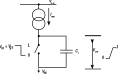
\includegraphics[width=3.5in]{ckt1.pdf}
\end{center}
& \nss \STT \\	
\end{longtable}

\end{document}
